\pagenumbering{gobble}

\normalfont\large
\medskip

\Large\fontspec{TradeWinds-Regular.ttf}The Evil
\normalfont\large
\medskip

What is special about your city? What makes it stand out compared to other cities? What makes it worth to protect? \rule{0.5\linewidth}{1pt}

\vspace{0.5cm}


\begin{tabular}{l @{\hspace{2cm}} l}
\Large\fontspec{TradeWinds-Regular.ttf}Type & \Large\fontspec{TradeWinds-Regular.ttf}They want to \\
\normalfont\large 1. Ninjas & \normalfont\large 1. Find and kill you \\
\normalfont\large 2. Aliens & \normalfont\large 2. Capture and experiment on you \\
\normalfont\large 3. Other mutants & \normalfont\large 3. Achieve (more) power\\
\normalfont\large 4. Scientists & \normalfont\large 4. Destroy the city\\
\normalfont\large 5. Regular human assholes & \normalfont\large 5. Get to your mentor\\
\normalfont\large 6. Occult forces & \normalfont\large 6. Prove their genius\medskip\\
\Large\fontspec{TradeWinds-Regular.ttf}They are a & \\
\normalfont\large 1. Clan & \normalfont\large \\ 
\normalfont\large 2. Cult & \normalfont\large \\ 
\normalfont\large 3. Enterprise & \normalfont\large \\ 
\normalfont\large 4. Family & \normalfont\large \\ 
\normalfont\large 5. Cartel & \normalfont\large \\ 
\normalfont\large 6. Secret society & \normalfont\large \medskip\\
\end{tabular}

\vspace{0.5cm}

\Large\fontspec{TradeWinds-Regular.ttf}~Example Enemies\medskip\\
\normalfont\large
\begin{tabular}{|l|l|l|l|}
    \hline
    Enemy Type & Harm & Damage & Notes \\
    \hline
    Grunt / Goon / Drone & 1--2 & 1 & Go down in a hit or two. Threat in numbers. \\
    \hline
    Thug / Mutant & 3 & 1--2 & More durable. May have strength or mutations. \\
    \hline
    Elite / Enforcer & 4 & 2 & Skilled fighters. Can briefly keep up with PCs. \\
    \hline
    Mini-Boss / Lieutenant & 5 & 2--3 & Dangerous. May have a unique move or mutation. \\
    \hline
    Boss / Major Villain & 6 & 3 & Serious threat. Might have armor or minions. \\
    \hline
    Omega-Level Threat & 7+ & 3--4 & Endgame danger. Requires teamwork or clever tactics. \\
    \hline
\end{tabular}

\vfill

\begin{tikzpicture}[remember picture, overlay]
  \node[anchor=south] at (current page.south) {
    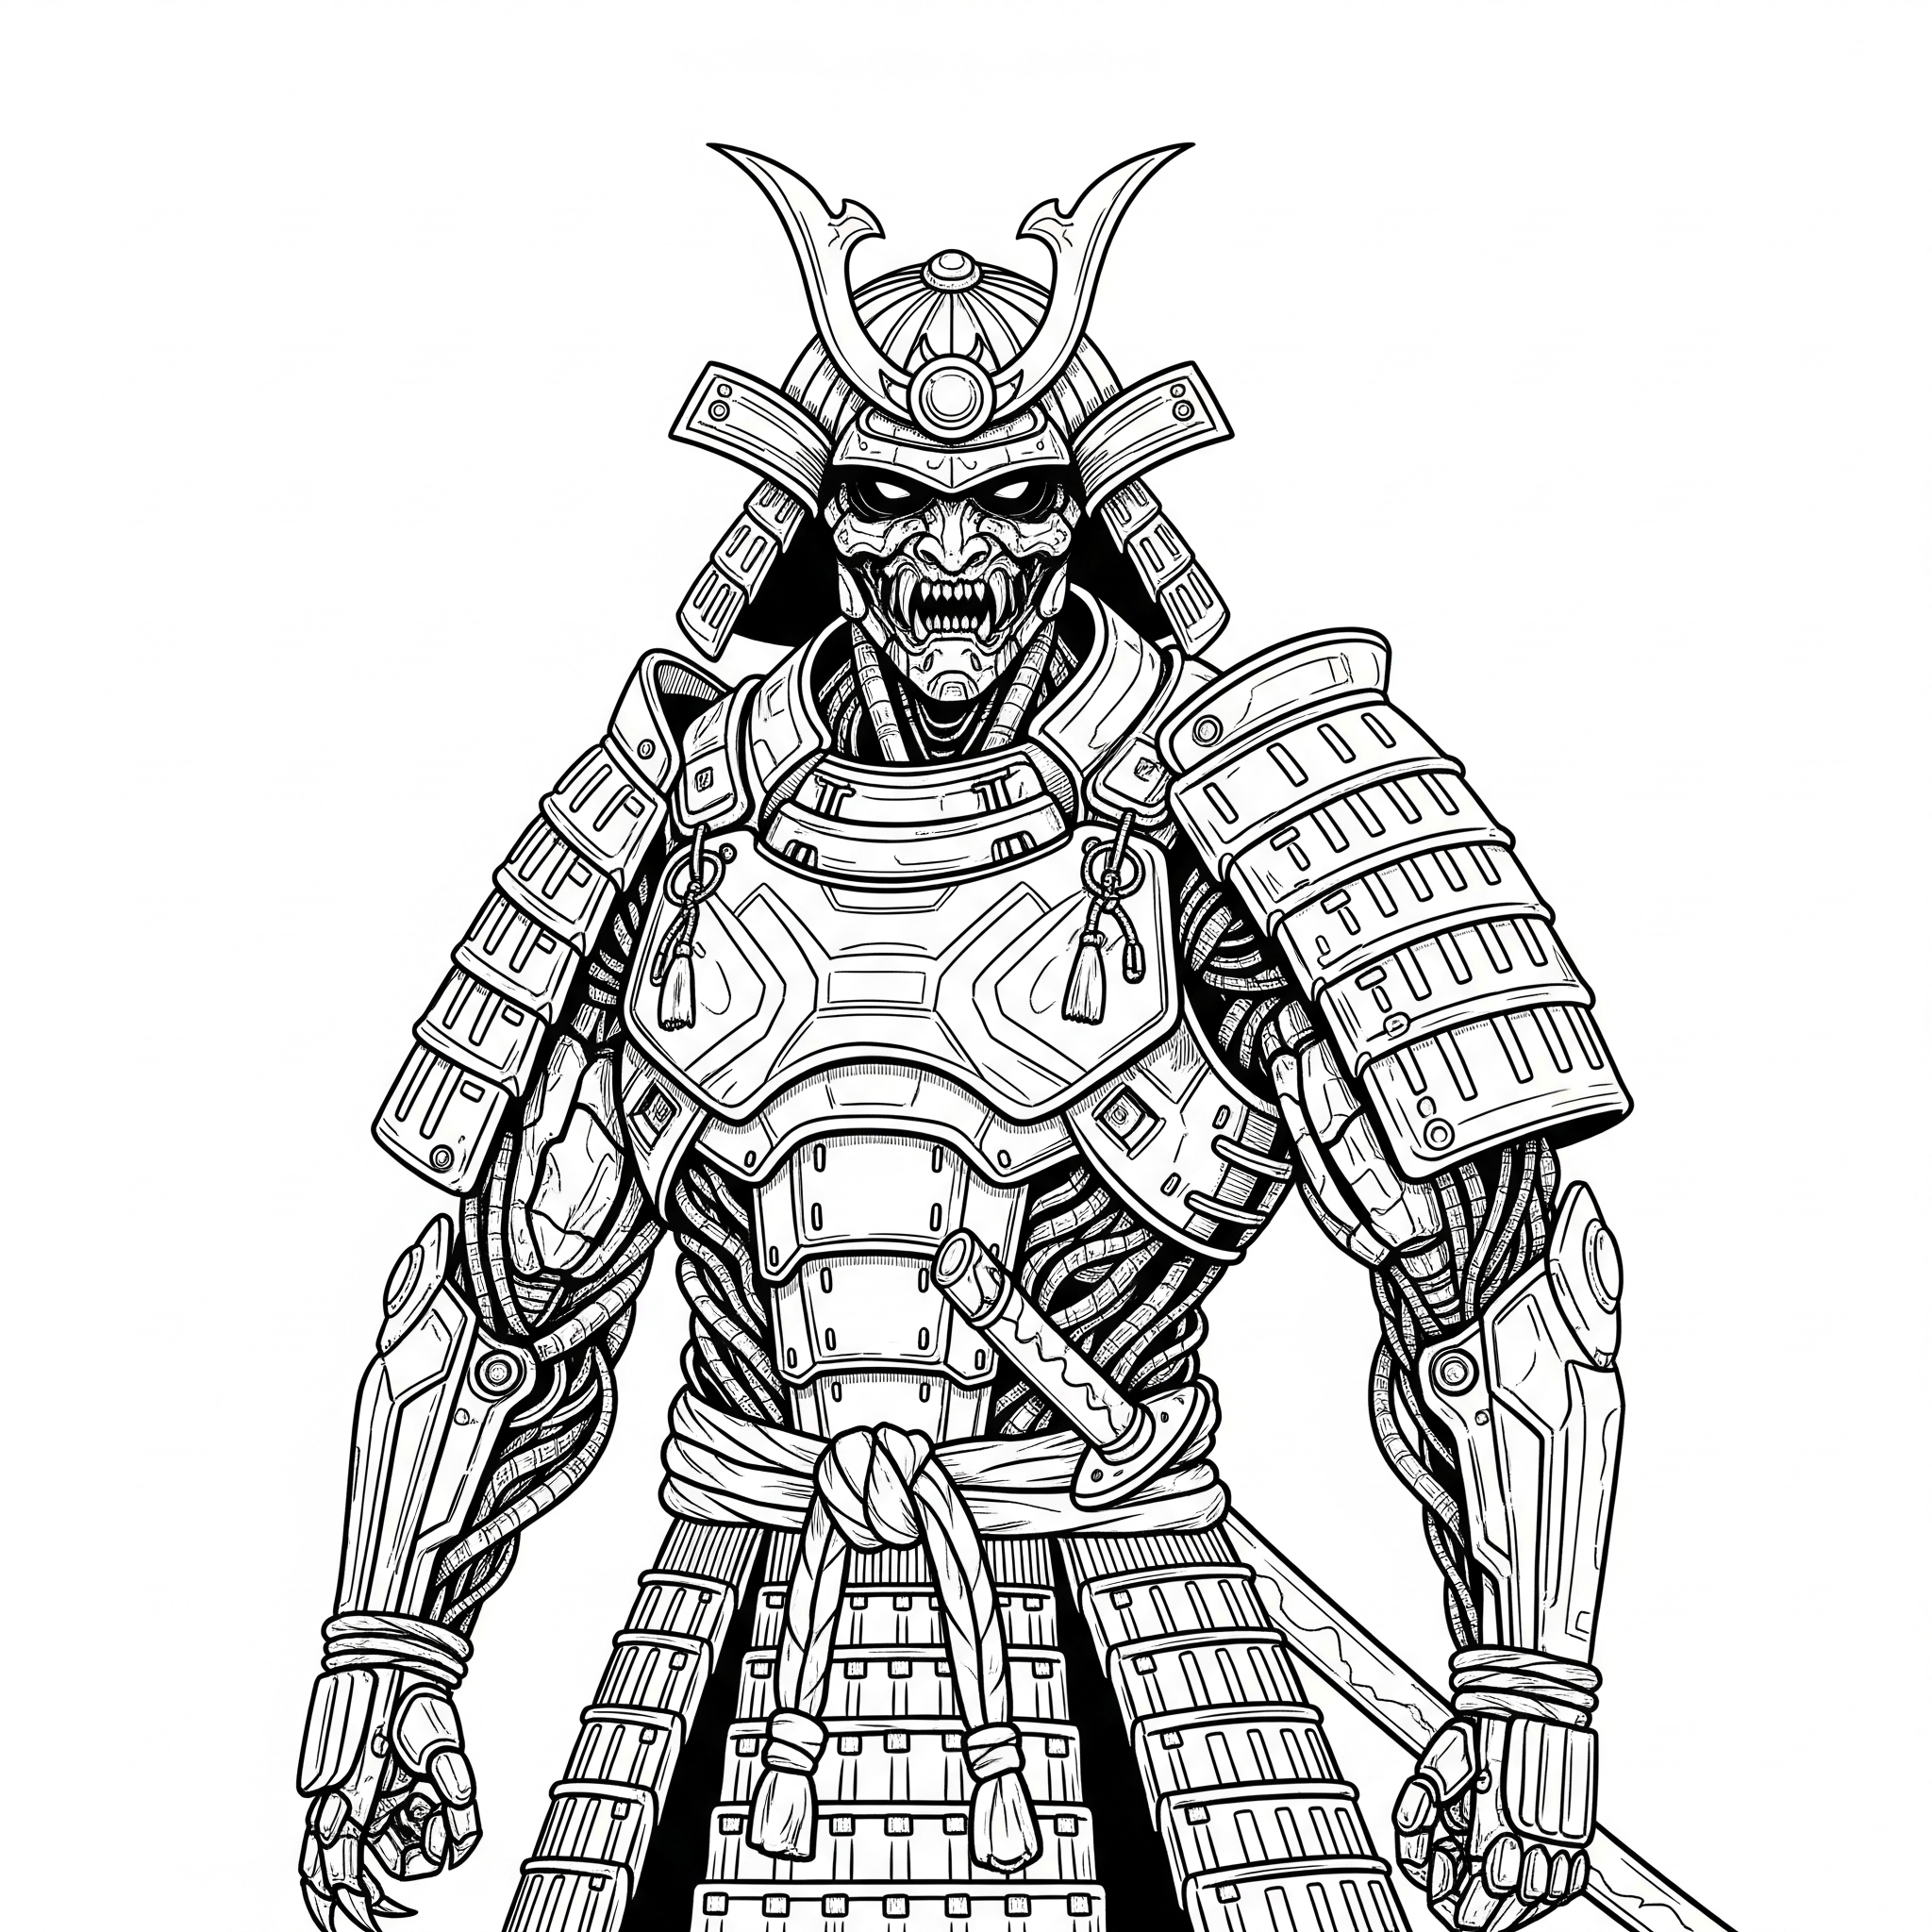
\includegraphics[height=9cm]{images/samurai.png}
  };
\end{tikzpicture}

\newpage